\begin{figure}[t]
\centering
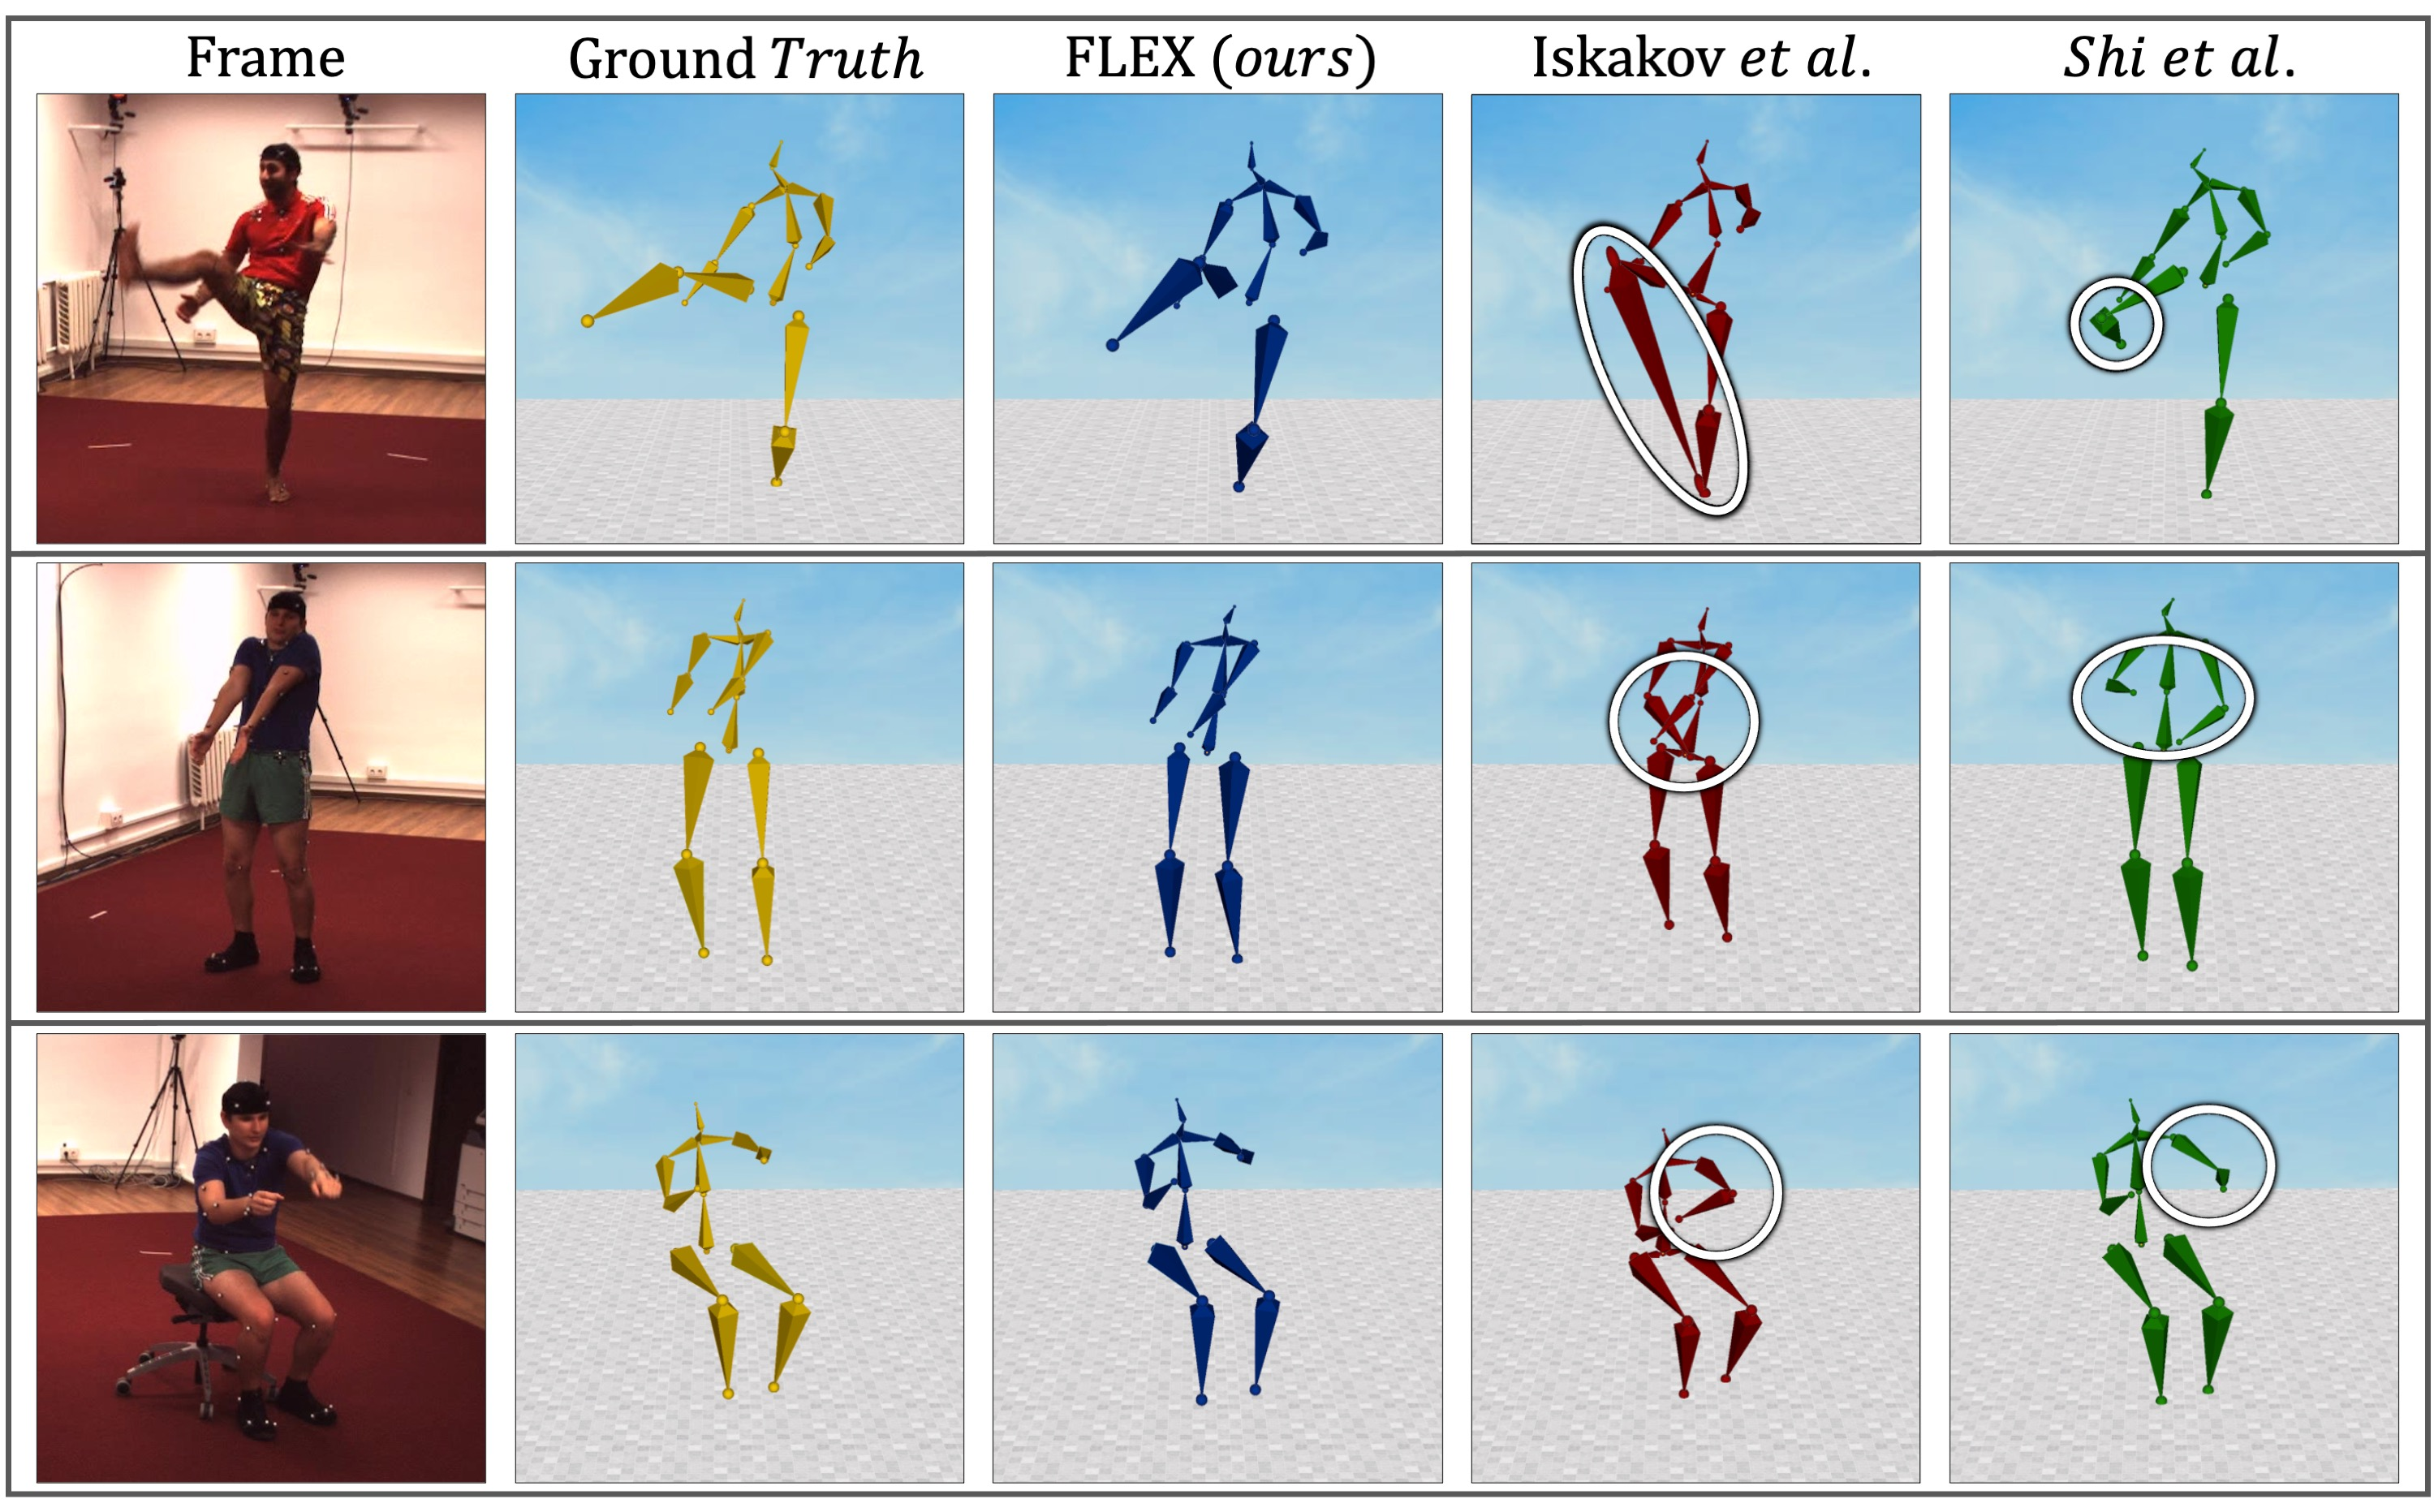
\includegraphics[width=\linewidth]{./images/competitors_grid.jpg}
\vspace{-20pt }
\caption{
%\color{orange}Frames from the H3.6M dataset. Shows the strenghts of our work. Predicting bones and rotations help to receive a more smooth motion. At Iskakvot \etal~\cite{iskakov2019learnable} column we can see the at the first row we received a huge right leg, and at the third colum the left elbow is rotated inside in a non-natural way. Comparing our results against Shi \etal~\cite{shi2020motionet} we show the benefits of our multi-view algorithm that produces more accurate results.}
Qualitative comparison of our work vs. non ep-free state-of-the-art (Iskakov \etal~\cite{iskakov2019learnable}) and vs. our single-view baseline (Shi \etal~\cite{shi2020motionet}).}
\label{fig:competitors}
\ifeccv
\else
\vspace{-17pt}
\fi
\end{figure}